\documentclass[tikz,border=5pt]{standalone}
\usepackage{pgfplots}
\pgfplotsset{compat=1.18}
\usetikzlibrary{decorations.pathreplacing}
\usepgfplotslibrary{fillbetween}
\usetikzlibrary{arrows.meta}

\definecolor{myCol}{HTML}{A4C7F0}
\definecolor{myCol2}{HTML}{C7F0A4}

\newcommand{\AxisRotator}[1][rotate=0]{%
\tikz[x=0.2cm,y=0.40cm,transform shape,#1]{%
    \draw[line width=0.5px,white,-] 
        (1.7,0.17) -- ++(0.55,0);

    % main arrow
    \draw[line width=0.2ex, -{Latex[length=2mm,width=1.2mm]}] 
        (0,0) arc (-170:170:1 and 1);
}}%

\begin{document}
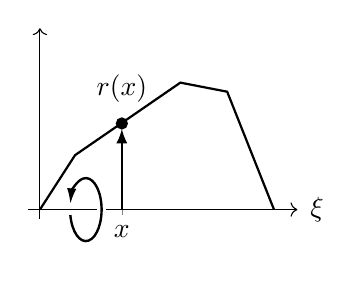
\begin{tikzpicture}
\begin{axis}[
    width=5cm,
    height=4cm,
    axis lines=middle,
    axis line style={->},
    xlabel={$\xi$},
    ylabel={},
    xlabel style={
        at={(axis description cs:0.95,0.05)},
        anchor=west,
        xshift=6pt
    },
    ylabel style={
        at={(axis description cs:0.05,0.95)},
        anchor=south,
        yshift=6pt
    },
    xmin=-0.1, xmax=2.2,
    ymin=-0.1, ymax=2,
    xtick={0,0.7},
    xticklabels={$0$,$x$},
    ytick=\empty,
    domain=0:2,
    samples=200,
    clip=false,
    legend style={draw=none, at={(0.02,0.95)}, anchor=west}
]

\addplot[thick, black] coordinates {
    (0.0, 0)
    (0.3, 0.6)
    (1.2, 1.4)
    (1.6, 1.3)
    (2.0, 0)
};

\addplot[only marks, mark=*, black] coordinates {
    (0.7,0.95)
};

%\node at (axis cs:2,0.8) {$r(\xi)$};

\draw[thick,->,-latex] (axis cs:0.7,0)  -- (axis cs:0.7,0.89) node[above,yshift=0.2cm] {$r(x)$};

\addplot[name path=axis, draw=none] 
    {0};

% \addplot[myCol] fill between[
%     of=curve and axis,
%     soft clip={domain=0:1.4}
% ];

% \addplot[myCol2] fill between[
%     of=curve and axis,
%     soft clip={domain=1.4:2}
% ];

\draw (0,0)  -- (2,0)  node [pos=0.2] {\AxisRotator};


\end{axis}
\end{tikzpicture}
\end{document}
